\section{Koordinatensysteme}

In diesem Kapitel werden wir sehen, wie wir in speziellen Koordinatensystemen bestimmte geometrische Objekte einfacher Darstellen können. Der Grund ist, das wir in der Computergrafik besser mit geraden Strecken rechnen können als mit kontinuierlichen Bögen. Die im Folgenden gezeigten Koordinatensysteme ermöglichen die Darstellung von rundungsintensiven Geometrien als Strecken oder n-Ecke. Dazu wird die Bedeutung der Achsen des kartesischen Koordinatensystems verändert.

\subsection{Polarkoordinatensystem}

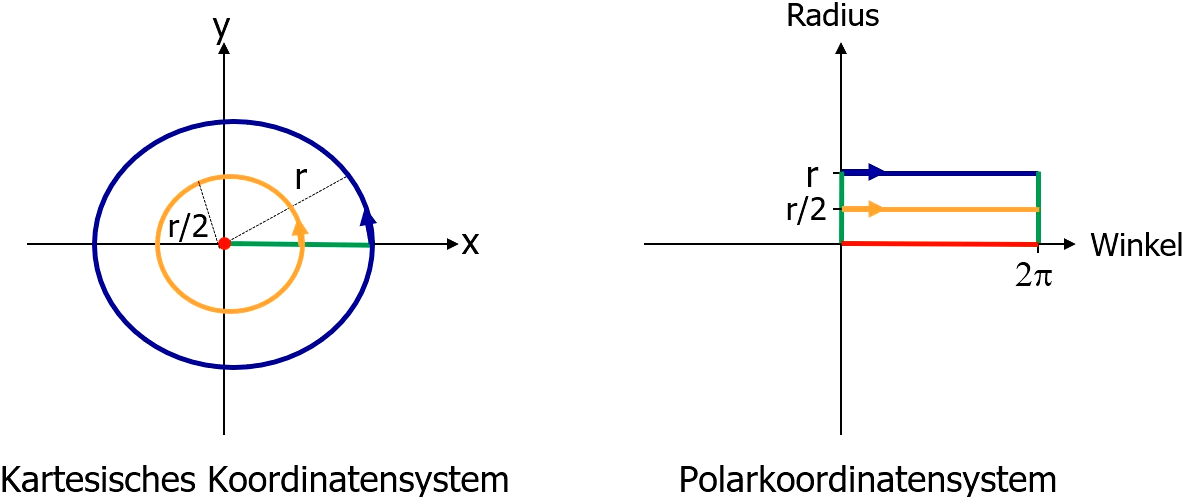
\includegraphics[width=400px]{Polarkoordinatensystem1.png}

Das Polarkoordinatensystem ist ein 2-dimensionales Koordinatensystem. Bei der Übertragung eines Punktes P aus dem kartesischen Koordinatensystems ins Polarkoordinatensystem wird die Entfernung des Punktes P zum Ursprung auf die eine Achse übertragen (Radius $r$). Auf die andere Achse wird der Winkel ($\alpha$) übertragen, den die positive x-Achse mit der Strecke zwischen dem Punkt P und dem Ursprung gegen den Uhrzeigersinn bildet. Dementsprechend sind die Umrechnungsregeln wie folgt definiert:\\

Von kartesischem Koordinatensystem zu Polarkoordinatensystem:\\
\begin{math}
    r = \sqrt{x^2 + y^2}\\
    \alpha = \arctan(y / x)
\end{math}

Von Polarkoordinatensystem zu kartesischem Koordinatensystem, mittels der Gesetzte für trigon. Funktionen entsprechend umgeformt, sodass die rechte Seite nur die Achsen des Polarkoordinatensystem enthält:\\
\begin{math}
    x = \cos{\alpha} \cdot r\\
    y = \sin(\alpha) \cdot r
\end{math}

Mittels dieser Definition können wir nun nun viele geometrische Formen, die normalerweise rundungen haben, als eckige Formen darstellen. Es folgt noch ein Beispiel.

\subsubsection{Kreisauschnitt im Polarkoordinatensystem}

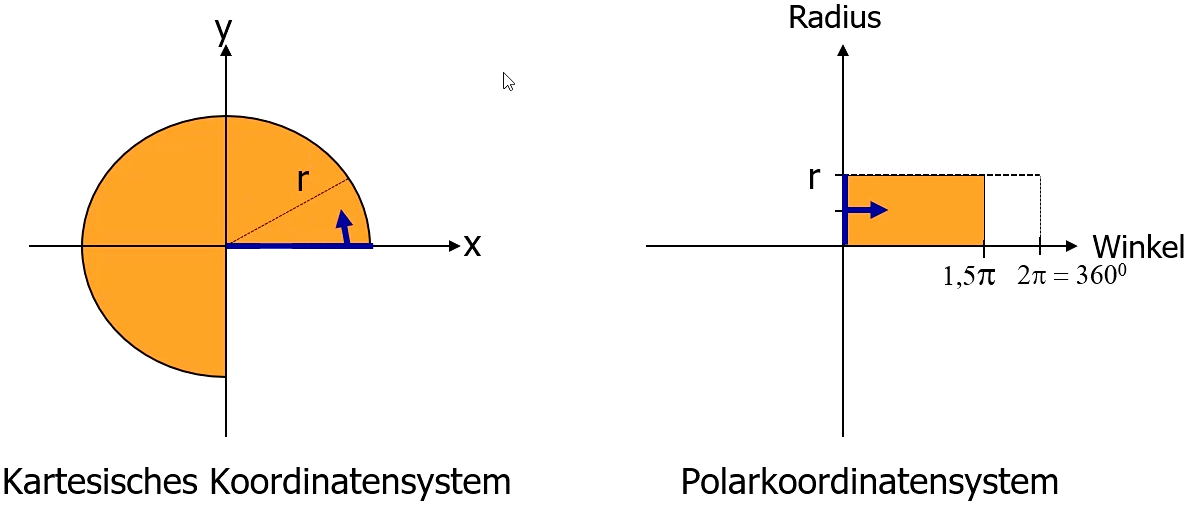
\includegraphics[width=350px]{Polarkoordinatensystem_Kreisausschnitte.png}


\subsection{Zylinderkoordinatensystem}

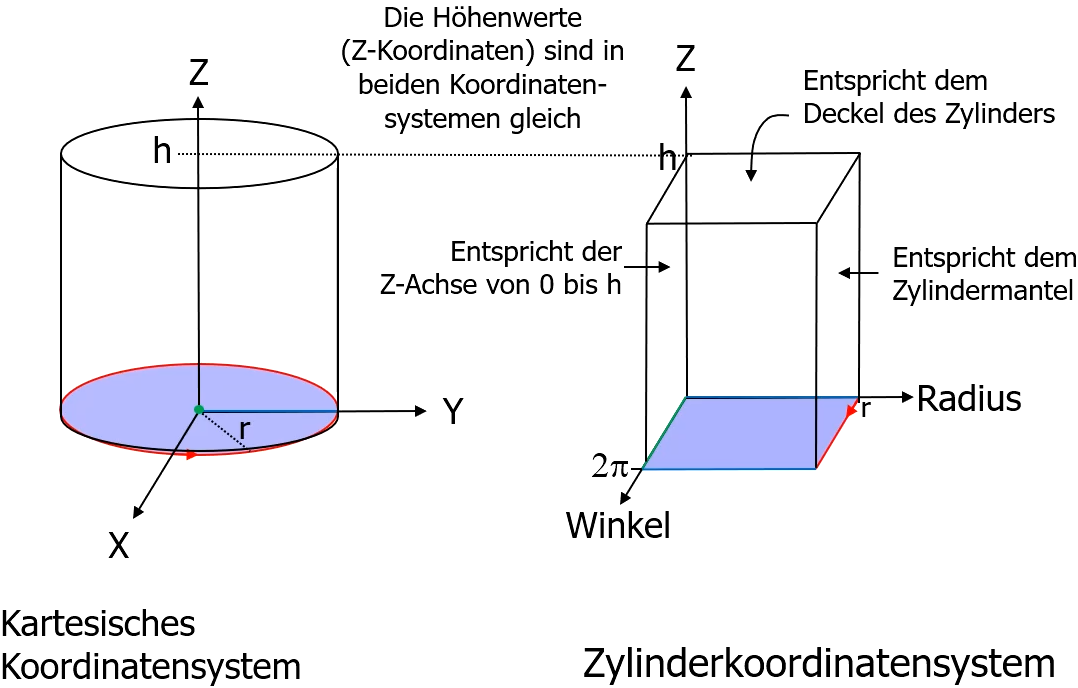
\includegraphics[width=350px]{Zylinderkoordinatensystem.png}

Das Zylinderkoordinatensystem ist ein 3-dimensionales Koordinatensystem, welches das Polarkoordinatensystem durch die z-Achse erweitert. Dabei ist die z-Achse unverändert so, wie sie auch im kartesischen Koordinatensystem ist. Somit ist die Umrechnung zwischen 3-dimensionalem kartesischen Koordinatensystem und Zylinderkoordinatensystem für x- und y-Koordinaten genau wie beim Umrechnen zwischen dem 2-dimensionalen kartesischen Koordinatensystem und dem Polarkoordinatensystem. Die z-Koordinate kann direkt übernommen werden.\\
Hier

\subsection{Kreiskoordinatensystem}

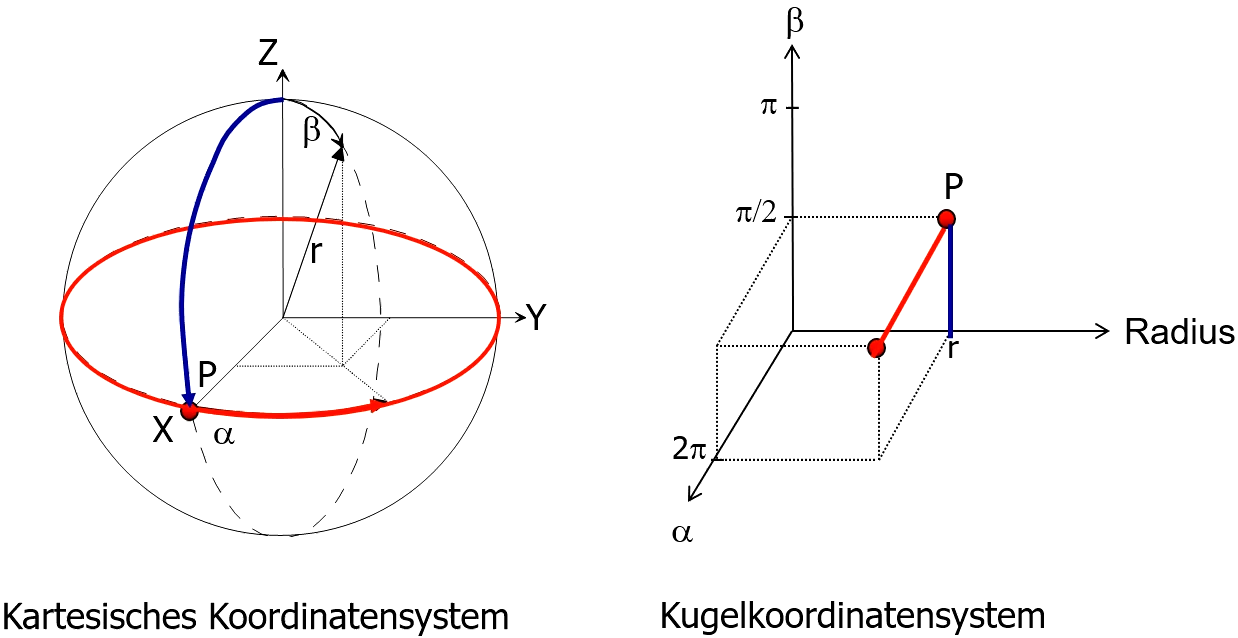
\includegraphics[width=400px]{Kugelkoordinatensystem.png}

Im Kreiskoordinatensystem wird die Position eines Punktes auf einer Kugeloberfläche mittels zweier Winkel $\alpha$ und $\beta$ beschrieben. Durch den Radius, der die Größe der Kugel bestimmt, kann dann jeder Punkt P im Raum beschrieben werden.\\
Einer der beiden Winkel (hier $\alpha$) muss $360°=2\pi$ abdecken. Der andere Winkel (hier $\beta$) muss nur $180°=pi$ abdecken. Denn, wenn wir die Linie, die von $\beta$ Bestimmt wird (hier in \textcolor{blue}{blau}) um den halben Kreis, also bis $\beta = 180°$ ziehen, können wir durch die Rotation um $\alpha = 360°$ (hier in \textcolor{red}{rot}) bereits die gesamte Oberfläche der Kugel abdecken.\\
Hier noch 2 Beispiele:\\
\\
\subsubsection{Äquatorebene im Kugelkoordinatensystem}
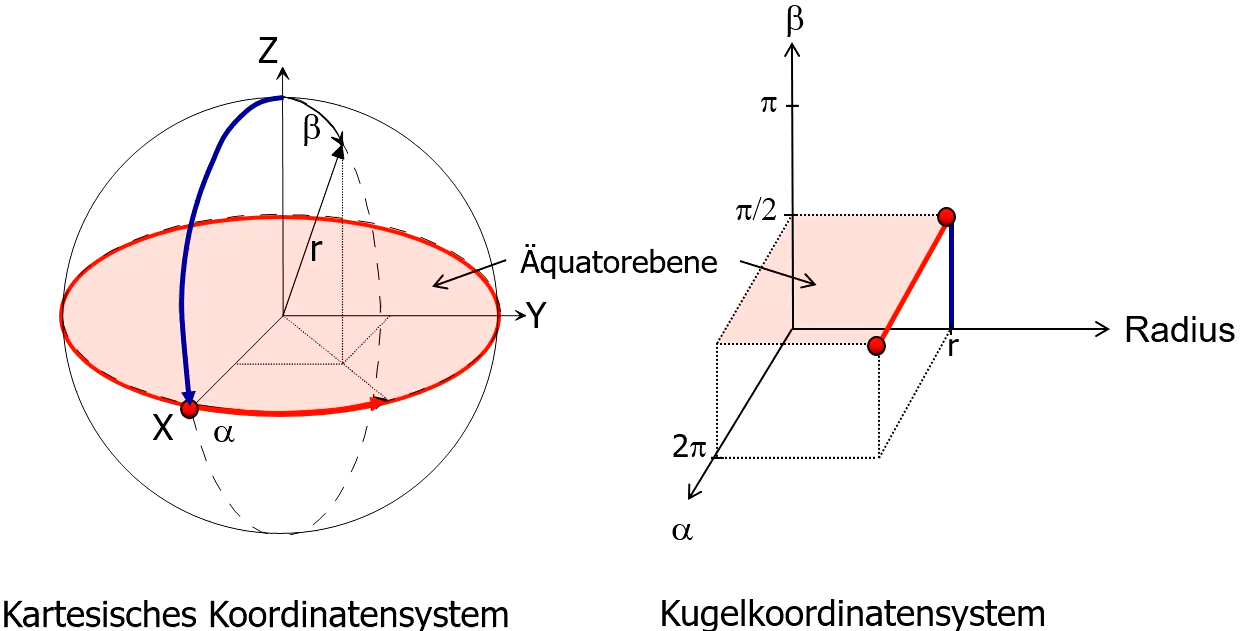
\includegraphics[width=300px]{Kugelkoordinatensystem_Aequatorebene.png}

\subsubsection{Halbkreise im Kugelkoordinatensystem}

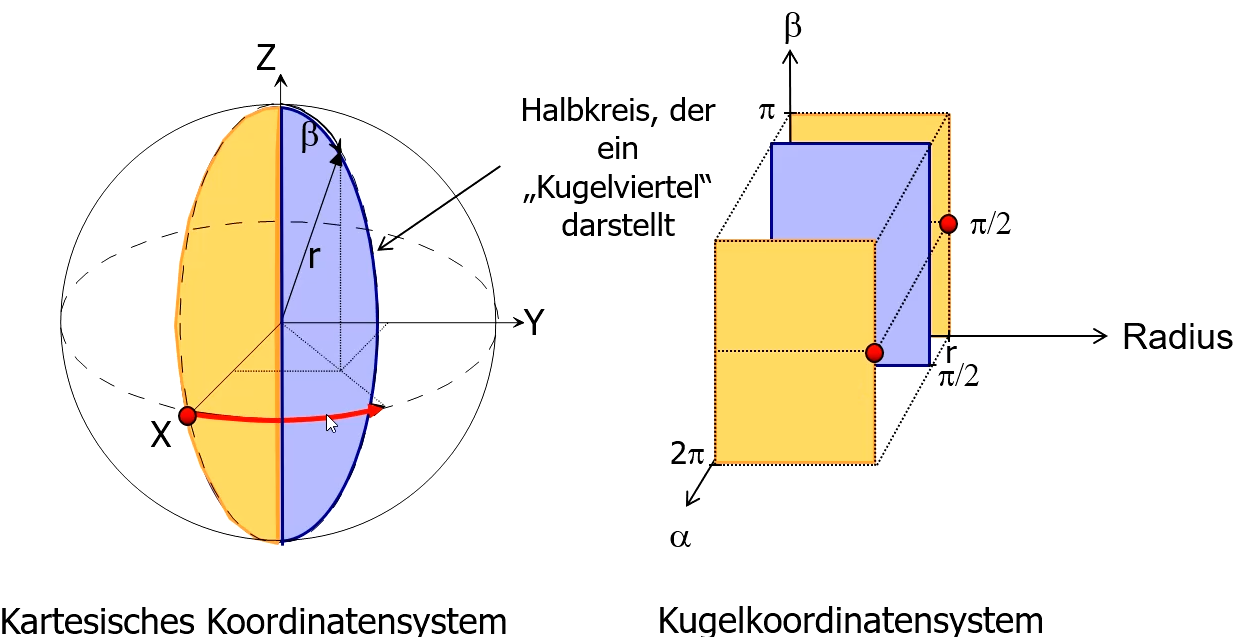
\includegraphics[width=300px]{Kugelkoordinatensystem_Halbkreis.png}
